\section{Decoder, basis, and arithmetic follow-ups}
\label{app:followup}

The decoder and matched-branch tests use the original architecture, data splits, and optimizer settings; operation and normalization controls are specified separately below. The basis study adds $52{,}698$ baseline updates and $9{,}000$ continuation updates. The subsequent causal study adds $364{,}302$ updates: five $24{,}000$-step arithmetic branches, fifteen $5{,}000$-step specificity branches, four original-trajectory extensions totaling $49{,}302$ steps, and four $30{,}000$-step operation or architecture controls. A subsequent horizon extension adds $420{,}000$ updates: each of the five corrected addition branches and the corrected subtraction run continues from step $30{,}000$ to $100{,}000$. The hidden-learning-rate control adds $470{,}000$ updates across five continuations from step $6{,}000$ to $100{,}000$. Verification replays are excluded from these totals. Multiple checkpoints and interventions from one trajectory are dependent observations.

\subsection{Monitoring and matched states}
\label{app:followup-protocol}

The causal branches and fresh baseline replications use a joint event: training and test accuracy must both fall below $90\%$ after sustained grokking. Training accuracy is checked at every update; test accuracy is checked every $100$ updates and at every post-grokking state with training accuracy below $90\%$. Thus every joint event is detected, while brief test-only excursions can fall between evaluations. Six consecutive grid evaluations at or above $95\%$ confirm grokking. The confirmation step is the \emph{last} evaluation of this six-check streak. Original sweep speeds instead report the start of a five-check streak (\S\ref{sec:setup}); the criteria therefore differ as well as their reporting points.

Within each seed, matched arithmetic branches restore identical parameters, optimizer buffers, and random-number-generator state. Exact next-update replays reproduce all three. The original prefixes combine historical evaluation grids with densely captured failures; their positive events establish binary incidence. We therefore compare event presence, without comparing their counts, durations, or historical minima against the uniformly monitored branches. The five trajectories were selected for mechanistic study and give no estimate of collapse prevalence over an unrestricted seed population.

\begin{table}[htbp]
\centering
\small
\caption{Test accuracy (\%) at adjacent captured failures. $h_0,W_0$ precede the update; $h_1,W_1$ follow it. Each head is evaluated with each feature state, without retraining. Original events are captured under mixed historical monitoring grids (Appendix~\ref{app:followup-protocol}).}
\label{tab:adjacent}
\begin{tabular}{lrrrr}
\toprule
Seed & Before: $W_0h_0$ & Old head: $W_0h_1$ & New head: $W_1h_0$ & After: $W_1h_1$ \\
\midrule
$0$ & $95.49$ & $96.39$ & $31.86$ & $31.87$ \\
$1$ & $94.14$ & $94.18$ & $13.56$ & $9.09$ \\
$2$ & $99.99$ & $100.00$ & $1.01$ & $0.93$ \\
$3$ & $89.54$ & $91.01$ & $50.80$ & $53.60$ \\
$4$ & $91.34$ & $98.66$ & $66.75$ & $66.33$ \\
\bottomrule
\end{tabular}
\end{table}

\subsection{Fresh decoders and the basis hypothesis}
\label{app:basis}

Fresh bias-free linear decoders are fitted to the raw final residual using only the original $3{,}830$ training examples. An uncentered SVD preconditioner retains all $128$ dimensions, with singular values floored at $10^{-6}$ of the largest. Each inner fit estimates its own preconditioner. A $20\%$ split of the training set selects an $L_2$ penalty on the preconditioned coefficients from $\{0,10^{-8},10^{-6},10^{-4},10^{-2}\}$ by validation cross-entropy; the selected decoder is then refitted on all training examples. The $8{,}939$ test examples enter only the final evaluation. Fits use float64 logistic regression and L-BFGS-B; convergence and unregularized controls are recorded.

At the selected collapsed checkpoints, decoder accuracies for seeds $0$--$4$ are $98.72\%$, $98.20\%$, $100.00\%$, $98.77\%$, and $100.00\%$, against $99.51\%$, $99.56\%$, $100.00\%$, $99.40\%$, and $100.00\%$ at their references. Probe checkpoints are steps $17{,}494$, $17{,}721$, $18{,}069$, $16{,}309$, and $16{,}060$: the last two occur after the adjacent transitions in Table~\ref{tab:adjacent}. These results establish substantial surviving linear task information; the small gaps in three seeds leave room for reduced decodability or probe limitations.

For column residuals, an exact global basis account requires one invertible $R$ satisfying $h_1(x)=Rh_0(x)$ across the operand grid. With examples stacked as rows, full column rank makes this equivalent to equality of the two feature column spaces. We test train-fitted linear and affine maps, centered reconstruction, rank sensitivity, principal angles, and a separately identified full-domain oracle. Centering by training means prevents a large constant feature component from dominating reconstruction error.

\begin{table}[htbp]
\centering
\small
\caption{Centered held-out reconstruction error (\%) for a train-fitted map from later to earlier residuals. Healthy controls match interval length. Reference intervals span $6$--$508$ updates and occur at different optimization stages, so comparisons are within each seed.}
\label{tab:followup-geometry}
\begin{tabular}{lrrr}
\toprule
Seed & \shortstack{Reference to\\captured failure} & Healthy interval & \shortstack{Adjacent\\failure update} \\
\midrule
$0$ & $43.63$ & $32.66$ & $1.88$ \\
$1$ & $43.05$ & $10.82$ & $4.63$ \\
$2$ & $9.05$ & $2.76$ & $1.10$ \\
$3$ & $45.73$ & $14.30$ & $10.66$ \\
$4$ & $25.60$ & $1.18$ & $25.63$ \\
\bottomrule
\end{tabular}
\end{table}

Positive controls plant exact residual gauges into the trained network. Eight controls cover condition numbers $1$, $3$, $10$, and $100$ in float32 and float64; twenty-four further controls plant observed fitted matrices with their measured orientation and conditioning. Exact compensation and train-fitted compensation recover $100\%$ in every fixed-condition control. For the three fresh adjacent transitions, observed forward-map errors are $4.65\%$, $1.10\%$, and $10.77\%$, against $0.0004$--$0.0006\%$ for their planted controls. These errors reject exact global equivalence for the measured pairs. Healthy evolution also departs from exact equivalence (Table~\ref{tab:followup-geometry}).

Approximate transport remains useful: inverse-linear compensation reaches $95.13\%$, $100\%$, and $94.37\%$ at the three fresh first events. Reference timing matters. Seed $0$'s head from step $17{,}200$ scores $14.05\%$ on the collapsed residual, while the head from $17{,}493$ scores $96.39\%$. Its geometric discrepancy from the distant reference is already present before the final failing update. Moreover, the complete real task-only Fourier coefficient matrices have shape $113\times128$; when both have full row rank, an invertible map between them always exists. For the seed-$4$ generalization-drop pair at steps $16{,}000$ and $17{,}000$, a fitted task-only map aligns that projection exactly while scoring $4.62\%$ on raw held-out features. This pair is separate from the adjacent failures above.

One-time repairs also have limited persistence. Eighteen continuations resume two captured failures for $500$ updates under nine head/state interventions each. Every successful repair retaining optimizer state falls below $90\%$ training accuracy on the next update. Clearing the head's Adam state improves eventual recovery but permits the immediate relapse. These tests separate instantaneous decodability from stability under continued optimization.

\subsection{Arithmetic interventions}
\label{app:arithmetic}

The accurate loss evaluates $\log(1+\sum_{j\ne y}\exp(z_j-z_y))$ with \texttt{log1p} whenever the correct-class logit is maximal; other examples use ordinary cross-entropy. Model storage, backward matrix arithmetic, and Muon's update remain float32. This avoids cancellation in the small loss and correct-class derivative, following the numerical concerns of \citet{prieto2025grokking}. All five step-$6{,}000$ sources already satisfy the six-check grokking criterion and already contain measurable gradient error. The intervention acts on an existing post-grokking trajectory.

\begin{table}[htbp]
\centering
\small
\caption{Matched arithmetic branches from step $6{,}000$ through $30{,}000$. Original columns show a captured joint failure. Accurate-CE branches have no joint failure; all finish at $100\%$ train and test accuracy. Minima include the starting state.}
\label{tab:followup-arithmetic}
\begin{tabular}{lrrr}
\toprule
Seed & Original event step & \shortstack{Original event\\test (\%)} & \shortstack{Accurate minimum\\test (\%)} \\
\midrule
$0$ & $17{,}494$ & $31.872$ & $99.754$ \\
$1$ & $17{,}721$ & $9.095$ & $99.843$ \\
$2$ & $18{,}069$ & $0.929$ & $98.859$ \\
$3$ & $16{,}308$ & $53.597$ & $99.978$ \\
$4$ & $16{,}056$ & $66.327$ & $99.843$ \\
\bottomrule
\end{tabular}
\end{table}

The specificity study branches each seed at step $15{,}000$ and runs to $20{,}000$ with three corrections. Accurate CE gives $0/5$ joint failures; target-derivative repair gives $0/5$; per-example zero-sum projection gives $0/5$. Every original trajectory has a captured failure in this window. All fifteen corrected branches finish at $100\%$ test accuracy; the minimum measured test accuracy across these branches is $99.978\%$.

For stock logit gradient $g$, target repair retains each wrong-class entry and sets $g_y=-\sum_{j\ne y}g_j$, leaving the reported forward loss unchanged. Projection replaces $g$ by $g-\mathbf{1}(\mathbf{1}^{\top}g)/p$. Both corrections compute their class sums in float64 and cast the result back to float32. Derivative errors are relative $L_2$ errors against the accurate float64 derivative evaluated on the identical float32 logits. The readout-gradient reference casts this logit derivative to float32 before backpropagating through the shared float32 network. At the fixed seed-$4$, step-$16{,}000$ audit, target repair reduces relative derivative error from $32.02\%$ to $4.19\times10^{-7}$, whereas projection leaves $31.88\%$. At step $20{,}000$, projected derivatives retain $52.94$--$86.07\%$ relative error despite a class-sum residual below $2.1\times10^{-8}$ relative to the reference norm. Thus restoring the class-sum identity can prevent the observed failures over this window even with substantial remaining derivative error. Numerical feature inflation and this projection control build on \citet{liu2026glitching}.

At step $15{,}000$, stock logit-gradient errors are $10.56$--$21.86\%$ and readout-gradient errors $18.95$--$43.42\%$. Passing a class-common gradient error through the same saved Adam state produces a class-centered update difference: its centered norm fraction is $45.85$--$73.37\%$, versus $(2.8$--$4.1)\times10^{-16}$ for scalar SGD, at float64 roundoff. These descriptive norm ratios are nonadditive. Accurate-CE branches also have smaller feature means: original mean norms at step $15{,}000$ are $2.22$--$3.83$ times their matched corrected values.

\textbf{Persistence through the original training horizon.} We resume each corrected step-$30{,}000$ state through step $100{,}000$, matching the original depth-$1$ horizon. All model parameters, optimizer buffers, and the PyTorch random state are restored. Twelve direct updates agree bitwise with both the monitored runner and a six-plus-six resumed continuation for all six sources. Each extension adds $70{,}000$ updates, with training accuracy recorded at every state and test accuracy every $100$ steps and whenever training accuracy is below $90\%$. The final and minimum-accuracy checkpoints reproduce their logged metrics exactly.

\begin{table}[htbp]
\centering\small
\caption{Corrected-loss runs through step $100{,}000$. Accuracies are percentages. Minima combine the earlier prefix with the extension, counting the shared step-$30{,}000$ state once. Addition is corrected from step $6{,}000$; subtraction uses corrected CE from initialization and its minima start at grokking confirmation.}
\label{tab:long-horizon}
\begin{tabular}{lrrrr}
\toprule
Run & Monitoring start & Min.\ test & Final test & Joint event \\
\midrule
Addition, seed 0 & $6{,}000$ & $99.754$ & $100.000$ & none \\
Addition, seed 1 & $6{,}000$ & $99.843$ & $100.000$ & none \\
Addition, seed 2 & $6{,}000$ & $98.859$ & $100.000$ & none \\
Addition, seed 3 & $6{,}000$ & $99.978$ & $100.000$ & none \\
Addition, seed 4 & $6{,}000$ & $99.843$ & $100.000$ & none \\
Subtraction, seed 0 & $10{,}500$ & $96.879$ & $99.955$ & none \\
\bottomrule
\end{tabular}
\end{table}

All six extensions complete without a joint event. Thus correction suppresses the observed failures through the original training budget. This addresses postponement beyond step $30{,}000$ within that budget; behavior after $100{,}000$ and brief test-only excursions between scheduled evaluations remain outside the measurement. The original stock trajectories already have captured failures by $30{,}000$, which establishes their positive binary incidence at the longer horizon. Their historical monitoring supports no comparison of event counts or durations with these dense branches.

\subsection{Mean amplification and finite-step overshoot}
\label{app:mean-update}

At the checkpoints immediately before the five original failures, feature means over the full operand grid have norms $10{,}374$--$12{,}203$. The main-text intervention in Eq.~\ref{eq:followup-mean} uses the post-update representation's training mean and adds each component to the rescued logits $W_{U,0}h_1$.
Applying the training-estimated mean unchanged to test examples, the mean term alone gives $32.11\%$, $9.42\%$, $0.93\%$, $53.34\%$, and $66.07\%$ accuracy, close to the full failing updates in Table~\ref{tab:followup-arithmetic}. The centered term alone retains $95.26\%$, $92.48\%$, $100\%$, $87.20\%$, and $98.46\%$. Relative reconstruction error is below $3\times10^{-16}$. This evaluation-only intervention establishes local sufficiency of the product of feature mean and readout displacement. Feature growth and optimizer history remain coupled before that step.

Replacing gradients only at the failing update with accurate gradients preserves all five failures. The state accumulated beforehand matters. For each actual complete parameter displacement $\Delta\theta$, the accurate training gradient satisfies $\nabla L^{\top}\Delta\theta<0$, including each group's contribution. Scaling the displacement by $0.001$ or $0.01$ lowers training loss in every seed; taking the full step raises it sharply. Both interpolation endpoints reproduce saved parameters exactly. The captured updates locally descend and overshoot at finite scale.

\subsection{Subtraction and normalized architecture}
\label{app:normalized}

Four additional runs use seed $0$ and a fixed $30{,}000$-step horizon: a stock/accurate-CE pair on subtraction and a pair on addition with gain-free RMS normalization before attention, before the MLP, and before the readout ($\epsilon=10^{-6}$). Parameter initialization and optimizer settings are matched, with no added parameters or hyperparameter search.

\begin{table}[htbp]
\centering
\small
\caption{Operation and architecture controls. Confirmation is the end of the six-check grokking streak. First-event test accuracies and post-grokking minima are separate measurements; both RMS runs subsequently recover to $100\%$. Each row is one seed.}
\label{tab:followup-generality}
\begin{tabular}{llrrrr}
\toprule
Condition & CE & Confirmation & First event & Event test (\%) & Min.\ test (\%) \\
\midrule
Subtraction & Stock & $9{,}300$ & $15{,}281$ & $5.851$ & $5.851$ \\
Subtraction & Accurate & $10{,}500$ & none & n/a & $96.879$ \\
RMS addition & Stock & $15{,}700$ & $18{,}515$ & $85.658$ & $0.481$ \\
RMS addition & Accurate & $19{,}900$ & $28{,}495$ & $0.884$ & $0.526$ \\
\bottomrule
\end{tabular}
\end{table}

Subtraction reproduces acute readout sensitivity: updated features with the preceding head score $98.81\%$, the mean term alone $5.84\%$, and the centered term $98.76\%$. At step $30{,}000$, accurate CE has no joint event and test accuracy is $99.966\%$. Its continuation through $100{,}000$ is reported in Table~\ref{tab:long-horizon}.

\begin{figure}[t]
\centering
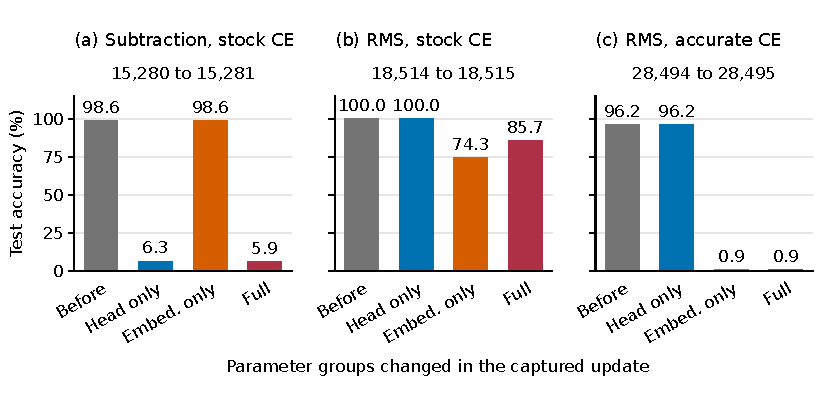
\includegraphics[width=\textwidth]{followup_rms_boundary.pdf}
\caption{One-step parameter interventions at the first detected joint failure in each operation or architecture control, all at seed $0$. Each bar uses the preceding checkpoint with only the indicated parameter group replaced by its following value; ``Full'' applies all three groups. In subtraction, the head update reproduces most of the damage. In both RMS cases, the embedding update is destructive while the head update preserves accuracy. The accurate-CE RMS failure occurs with an accurate loss derivative. These are first-event measurements at the displayed steps; the later post-grokking minima are reported separately in Table~\ref{tab:followup-generality}.}
\label{fig:followup-rms}
\end{figure}

In the RMS runs, the embedding update causes the acute loss of accuracy. In the accurate-CE event, test accuracy falls from $96.208\%$ to $0.884\%$; its logit derivative has relative error $9.48\times10^{-8}$ and no vanished correct-class entries. Updating only the head retains $96.208\%$, updating only embeddings gives $0.940\%$, and freezing the head still gives $0.895\%$. The minimum reaches $0.526\%$ at step $28{,}503$; the stock-RMS minimum is $0.481\%$ at $28{,}540$. Exact update replay passes. Both RMS event directions locally descend and lower loss at scales $0.001$ and $0.01$, then overshoot at full scale. This counterexample bounds the readout/feature-mean account to the measured unnormalized cases and rules out universal prevention by accurate loss arithmetic. The completed horizons support those finite claims; longer runs and population frequencies remain outside their scope.

\clearpage
\subsection{Post-grokking hidden-learning-rate reduction}
\label{app:lr-reduction}

We restore the same five original step-$6{,}000$ checkpoints used for the arithmetic branches, including the full model, optimizer buffers, and random-number-generator state. Immediately after restoration, we reduce the hidden Muon learning rate from $0.03$ to $0.003$ and hold it fixed through step $100{,}000$. Embeddings and readout remain trainable at learning rates $0.001$ and $0.00025$, respectively. All branches retain stock cross-entropy and the original weight-decay coefficients: $0.1$ for the hidden matrices and $1$ for embeddings and readout. Each continuation adds $94{,}000$ updates, for $470{,}000$ in total.

The primary outcome is whether a seed has any state with both training and held-out test accuracy below $90\%$. Training accuracy is recorded at every update, including the source and final states. Test accuracy is evaluated every $100$ updates and whenever training accuracy is below $90\%$, matching the corrected-loss protocol. This gives $94{,}001$ recorded training states per seed. Test-only excursions between scheduled evaluations can be missed.

\begin{table}[htbp]
\centering\small
\caption{Hidden-LR continuations through step $100{,}000$. Every seed has a joint failure. Test accuracies are percentages, and minima include the starting state. Below-$95\%$ counts include all test evaluations under the stated monitoring rule; the scheduled subset uses only the $100$-step grid. These counts describe the new branches.}
\label{tab:lr-reduction}
\begin{tabular}{lrrrrr}
\toprule
Seed & \shortstack{First joint\\failure step} & \shortstack{Minimum\\sampled test} & \shortstack{Evaluations\\below $95\%$} & \shortstack{Scheduled\\subset} & Final test \\
\midrule
$0$ & $18{,}767$ & $0.8614$ & $105$ & $13$ & $100.0000$ \\
$1$ & $18{,}476$ & $4.7209$ & $88$ & $20$ & $100.0000$ \\
$2$ & $19{,}439$ & $0.8950$ & $135$ & $14$ & $99.6644$ \\
$3$ & $17{,}041$ & $4.8999$ & $52$ & $22$ & $99.8881$ \\
$4$ & $17{,}578$ & $0.8166$ & $103$ & $13$ & $100.0000$ \\
\bottomrule
\end{tabular}
\end{table}

All five reduced-LR branches experience a joint failure, compared with $5/5$ original stock trajectories and $0/5$ corrected-loss branches through the same horizon. We compare binary seed-level incidence because the original trajectories have different historical monitoring. The reduced-LR branches first fail between steps $17{,}041$ and $19{,}439$; seeds $0$, $2$, and $4$ reach approximately chance-level test accuracy ($1/113\approx0.885\%$). All recover to at least $99.6644\%$ final test accuracy. Their recovery illustrates why final accuracy alone misses these failures.

\clearpage
\begin{table}[!htbp]
\centering\small
\caption{Sampled diagnostics for the hidden-LR branches. Each seed has $95$ measurements at $1{,}000$-step intervals, including steps $6{,}000$ and $100{,}000$. Feature means cover the full operand grid. CE error is the relative $L_2$ error of the stock float32 training-logit derivative against the accurate float64 derivative at the same logits, expressed as a percentage. Maxima are over the sampled diagnostic states.}
\label{tab:lr-reduction-diagnostics}
\begin{tabular}{lrrrrrr}
\toprule
& \multicolumn{3}{c}{Feature-mean norm} & \multicolumn{3}{c}{CE derivative error (\%)} \\
\cmidrule(lr){2-4}\cmidrule(lr){5-7}
Seed & Start & Final & Maximum & Start & Final & Maximum \\
\midrule
$0$ & $310.8$ & $292.6$ & $4{,}282.5$ & $1.440$ & $0.030$ & $38.558$ \\
$1$ & $459.5$ & $505.3$ & $8{,}783.8$ & $1.500$ & $0.180$ & $46.273$ \\
$2$ & $355.1$ & $1{,}096.5$ & $8{,}100.4$ & $0.967$ & $22.837$ & $36.585$ \\
$3$ & $411.9$ & $955.8$ & $8{,}878.5$ & $2.228$ & $5.408$ & $48.431$ \\
$4$ & $434.1$ & $445.1$ & $3{,}596.0$ & $1.748$ & $0.027$ & $63.645$ \\
\bottomrule
\end{tabular}
\end{table}

Every reduced-LR branch exhibits substantial feature-mean growth and loss-derivative error at sampled states (Table~\ref{tab:lr-reduction-diagnostics}). The accompanying artifacts retain training-set feature means, raw trajectories, checkpoint replays, and the detailed audits. We have not localized the parameter group responsible for these reduced-LR failures, so the evidence establishes joint failure without attributing it to the acute readout mechanism identified in the original branches. Ordinary learning-rate reduction also scales the decoupled weight-decay step: the hidden per-update decay factor changes from $1-0.03\times0.1=0.997$ to $1-0.003\times0.1=0.9997$. The tested tenfold reduction is therefore a stabilization control. It is insufficient to provide the stability achieved by corrected loss arithmetic for these five matched continuations through step $100{,}000$.
